\documentclass[11pt, a4paper]{article}

\usepackage{tikz}
\usetikzlibrary{shapes,arrows}
\usepackage{amsmath}
\usepackage{placeins}
\usepackage{amssymb}

\begin{document}

\title{PRINCIPAL COMPONENT ANALYSIS}
\date{}
\maketitle

Principal Component Analysis (PCA) is non-parametric approach to transform a set of observations - of possibly correlated variables - into another set of values defined by a calculated set of new orthogonal uncorrelated variables called principal components. 

\section{Example}

Consider the following set of four observations in two dimesions,

\begin{figure}[htbp]
	\centering
	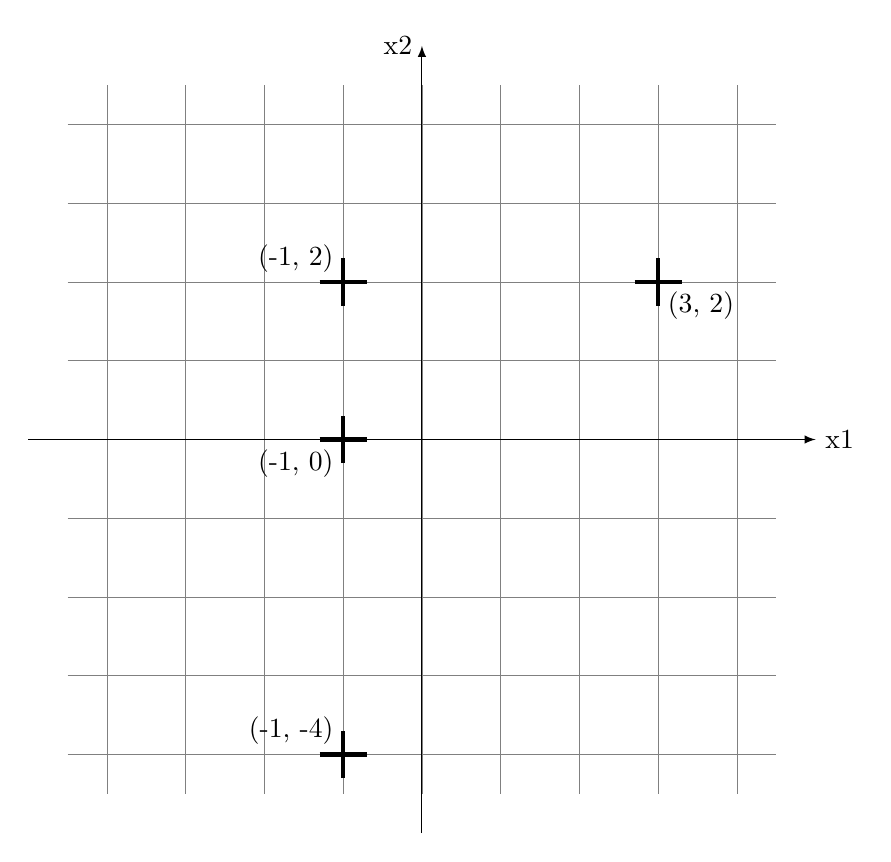
\begin{tikzpicture}
		\tikzstyle {point line} = [line width=0.15em]
		\tikzstyle {margin} = [dashed]
						
		\draw[step=1.0, gray, very thin] (-4.5, -4.5) grid (4.5, 4.5);
										    
		\draw[-latex] (-5,0) -- (5,0) node[right]{x1};
		\draw[-latex] (0,-5) -- (0,5) node[left]{x2};	
								
		\draw[point line] (2.7, 2) -- (3.3, 2);	
		\draw[point line] (3, 1.7) -- (3, 2.3);
		\draw (3, 2) node [below right] {(3, 2)};    	
						
		\draw[point line] (-1.3, 0) -- (-0.7, 0);	
		\draw[point line] (-1, -0.3) -- (-1, 0.3);	
		\draw (-1, 0) node [below left] {(-1, 0)};   
						
		\draw[point line] (-1.3, 2) -- (-0.7, 2);	
		\draw[point line] (-1, 1.7) -- (-1, 2.3);	
		\draw (-1, 2) node [above left] {(-1, 2)};   
						
		\draw[point line] (-1.3, -4) -- (-0.7, -4);	
		\draw[point line] (-1, -4.3) -- (-1, -3.7);	
		\draw (-1, -4) node [above left] {(-1, -4)};   
							   		
	\end{tikzpicture}
\end{figure}

To see how PCA alters the representation of this tiny dataset, the dataset is first written in matrix form as follows,

\begin{align*}
	X & = \begin{pmatrix} 3 & -1 & -1 & -1 \\
	2 & 0 & 2 & -4  
	\end{pmatrix}
\end{align*}

The x-axis intercepts are represented by the first row of this matrix while y-axis intercepts are represented by the second row.
This matrix can be thought of as a representation composed of two random variables x1 and x2. The variances of these variables and their covariance are useful quantities to describe the structure of the dataset.

\begin{align*}
	Var(x1)     & = \frac{1}{N} \sum\limits_{i = 1}^N (x1_i - \bar{x1})^2                \\
	            & = \frac{1}{4} \sum\limits_{i = 1}^4 (x1_i - 0)^2                       \\
	            & = \frac{1}{4} |x1|^2                                                   \\
	            & = \frac{3^2 + (-1)^ 2 + (-1)^2 + (-1)^2}{4}                            \\
	            & = 3                                                                    \\
	Var(x2)     & = \frac{1}{4} \sum\limits_{i = 1}^4 (x2_i - 0)^2                       \\
	            & = \frac{1}{4} |x2|^2                                                   \\
	            & = \frac{2^2 + 0^ 2 + 2^2 + (-4)^2}{4}                                  \\           
	            & = 6                                                                    \\
	Cov(x1, x2) & = \frac{1}{N} \sum\limits_{i = 1}^N (x1_i - \bar{x1})(x2_i - \bar{x2}) \\
	            & = \frac{1}{4} \sum\limits_{i = 1}^4 (x1_i - 0)(x2_i - 0)               \\  
	            & = \frac{1}{4} \vec{x1}.\vec{x2}                                        \\
	            & = \frac{3*2 + (-1)*0 + (-1)*2 + (-1)*(-4)}{4}                          \\
	            & = 2                                                                    
\end{align*}

Note that the mean of both the vectors is zero in the dataset. This is a necessary precondition for PCA, the reason for this constraint will become apparent in later sections. Next, these variances and covariance are arranged in a matrix as follows.

\begin{align*}
	\sum & = \begin{pmatrix} Var(x1) & Cov(x1, x2) \\
	Cov(x1, x2) & Var(x2) \\ 
	\end{pmatrix} \\
	     & = \begin{pmatrix} 3       & 2           \\
	2 & 6 \\ 
	\end{pmatrix}           
\end{align*}

Due to zero mean constraint, the following also holds true,

\begin{align*}
	\sum = \frac{1}{N} XX^T \\
\end{align*}

Now eigenvalues and eigenvectors of $\sum$ are calculated.

\begin{align*}
	\sum \phi              & = \lambda \phi \\
	(\sum - \lambda I)\phi & = 0            
\end{align*}

$(\sum - \lambda I)$ must be singular if eigenvectors are non-zero. Hence,

\begin{align*}
	\begin{vmatrix} 3 - \lambda & 2           \\
	2                           & 6 - \lambda \\ 
	\end{vmatrix}               & = 0         \\
	(3 - \lambda)(6 - \lambda)  & = 4         \\	                
\end{align*}

This gives eigenvalues $\lambda = 2, 7$ and eignevectors $\phi = (\frac{-2}{\sqrt{5}}, \frac{1}{\sqrt{5}}), (\frac{1}{\sqrt{5}}, \frac{2}{\sqrt{5}}) $ respectively. Now the eigenvectors are arranged as rows in a matrix in order of their corresponding eigenvalue. 


\begin{align*}
	P & = \begin{pmatrix} \frac{1}{\sqrt{5}}   & \frac{2}{\sqrt{5}} \\
	\frac{-2}{\sqrt{5}} & \frac{1}{\sqrt{5}} \\ 
	\end{pmatrix}  \\
	  & = \frac{1}{\sqrt{5}} \begin{pmatrix} 1 & 2                  \\
	-2 & 1\\ 
	\end{pmatrix}	                
\end{align*}


See the following visualization of eigenvectors.

\FloatBarrier\clearpage
\begin{figure}[htbp]
	\centering
	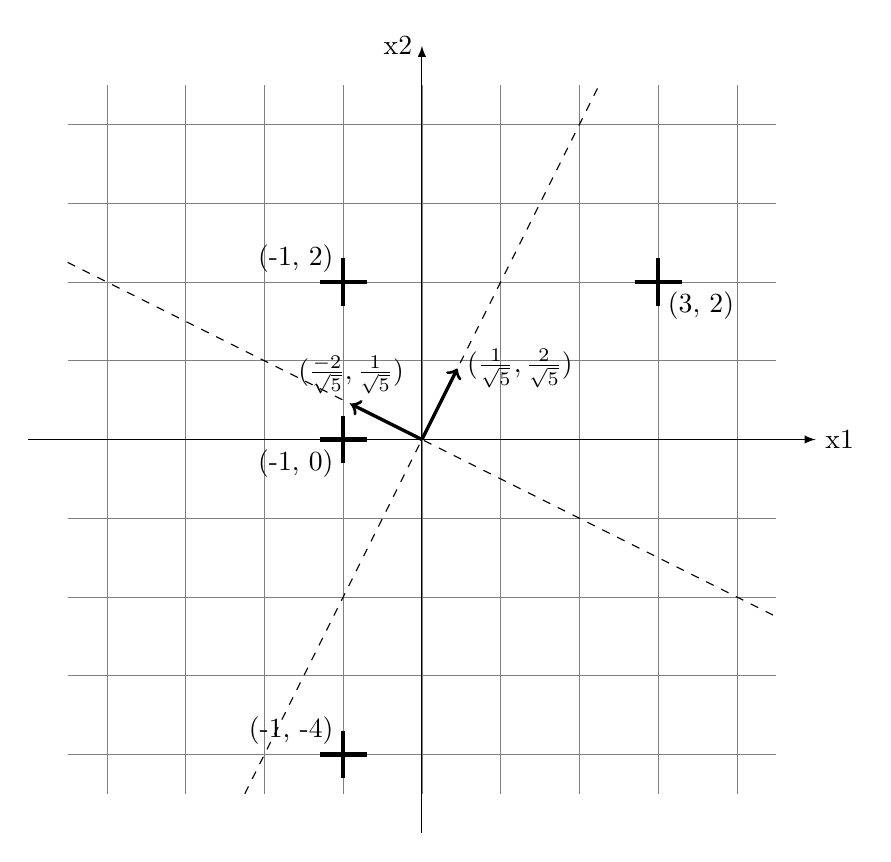
\begin{tikzpicture}
		\tikzstyle {point line} = [line width=0.15em]
		\tikzstyle {margin} = [dashed]
						
		\draw[step=1.0, gray, very thin] (-4.5, -4.5) grid (4.5, 4.5);
										    
		\draw[-latex] (-5,0) -- (5,0) node[right]{x1};
		\draw[-latex] (0,-5) -- (0,5) node[left]{x2};	
								
		\draw[point line] (2.7, 2) -- (3.3, 2);	
		\draw[point line] (3, 1.7) -- (3, 2.3);
		\draw (3, 2) node [below right] {(3, 2)};    	
						
		\draw[point line] (-1.3, 0) -- (-0.7, 0);	
		\draw[point line] (-1, -0.3) -- (-1, 0.3);	
		\draw (-1, 0) node [below left] {(-1, 0)};   
						
		\draw[point line] (-1.3, 2) -- (-0.7, 2);	
		\draw[point line] (-1, 1.7) -- (-1, 2.3);	
		\draw (-1, 2) node [above left] {(-1, 2)};   
						
		\draw[point line] (-1.3, -4) -- (-0.7, -4);	
		\draw[point line] (-1, -4.3) -- (-1, -3.7);	
		\draw (-1, -4) node [above left] {(-1, -4)}; 
				
		\draw[very thick,->] (0,0) -- (.45,.90);  
		\draw[dashed] (-2.25, -4.5) -- (2.25,4.5);
		\draw (.45, .90) node [right] {$(\frac{1}{\sqrt{5}}, \frac{2}{\sqrt{5}})$}; 
				
		\draw[very thick,->] (0,0) -- (-0.90,0.45);  
		\draw[dashed] (-4.5, 2.25) -- (4.5,-2.25);
		\draw (-0.90,0.45) node [above] {$(\frac{-2}{\sqrt{5}}, \frac{1}{\sqrt{5}})$};
							   		
	\end{tikzpicture}
\end{figure}

Now the transformed dataset Y is calculated simply as product of P and X.

\begin{align*}
	P &= \frac{1}{\sqrt{5}} \begin{pmatrix} 1 & 2 \\
	-2 & 1\\ 
	\end{pmatrix} \begin{pmatrix} 3 & -1 & -1 & -1 \\
	2 & 0 & 2 & -4  
	\end{pmatrix} \\ 
	  & = \frac{1}{\sqrt{5}} \begin{pmatrix} 7 & -1 & 3 & -9 \\
	-4 & 2 & 4 & -2  
	\end{pmatrix}
\end{align*}

To visualize the result, Y is plotted on a graph,

\FloatBarrier\clearpage
\begin{figure}[htbp]
	\centering
	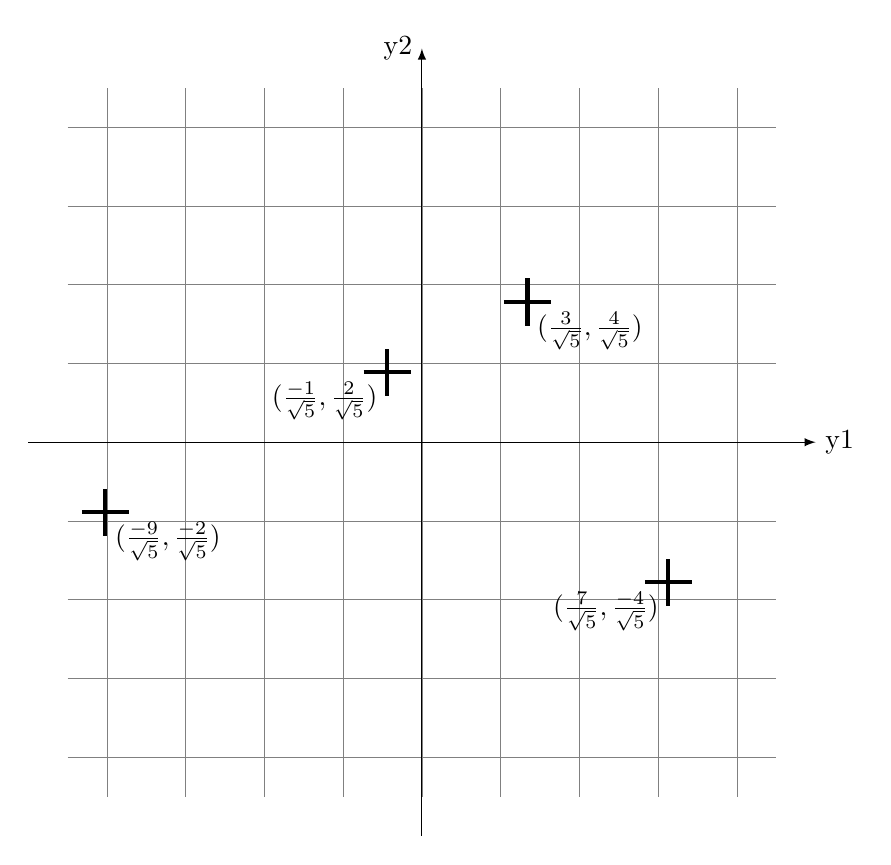
\begin{tikzpicture}
		\tikzstyle {point line} = [line width=0.15em]
		\tikzstyle {margin} = [dashed]
						
		\draw[step=1.0, gray, very thin] (-4.5, -4.5) grid (4.5, 4.5);
										    
		\draw[-latex] (-5,0) -- (5,0) node[right]{y1};
		\draw[-latex] (0,-5) -- (0,5) node[left]{y2};	
								
		\draw[point line] (2.83, -1.78) -- (3.43, -1.78);	
		\draw[point line] (3.13, -2.08) -- (3.13, -1.48);
		\draw (3.13, -1.78) node [below left] {$(\frac{7}{\sqrt{5}}, \frac{-4}{\sqrt{5}})$};    	
						
		\draw[point line] (-0.74, 0.89) -- (-0.14, 0.89);	
		\draw[point line] (-0.44, 0.59) -- (-0.44, 1.19);	
		\draw (-0.44, 0.89) node [below left] {$(\frac{-1}{\sqrt{5}}, \frac{2}{\sqrt{5}})$};   
						
		\draw[point line] (1.04, 1.78) -- (1.64, 1.78);	
		\draw[point line] (1.34, 1.48) -- (1.34, 2.08);	
		\draw (1.34, 1.78) node [below right] {$(\frac{3}{\sqrt{5}}, \frac{4}{\sqrt{5}})$};   
						
		\draw[point line] (-4.32 , -0.89) -- (-3.72 , -0.89);	
		\draw[point line] (-4.02, -1.19) -- (-4.02,-0.59 );	
		\draw (-4.02, -0.89) node [below right] {$(\frac{-9}{\sqrt{5}}, \frac{-2}{\sqrt{5}})$};   
							   		
	\end{tikzpicture}
\end{figure}

Visually, the points on the transformed graph arise due to a change of axes from the original axes to the axes defined by the eigenvectors of $\sum$. To see why this choice of axes was made, the variance covariance matrix of the transformed data is calculated.

\begin{align*}
	\sum_{new} &= \frac{1}{N} YY^T \\
	  & = \frac{1}{4} \frac{1}{\sqrt{5}} \begin{pmatrix} 7 & -1 & 3 & -9 \\
	-4 & 2 & 4 & -2  
	\end{pmatrix} \frac{1}{\sqrt{5}}  \begin{pmatrix} 7 & -4 \\
	-1 & 2 \\
	3 & 4 \\
	-9 & -2 \\   
	\end{pmatrix} \\
	&=  \frac{1}{20} \begin{pmatrix} 140 & 0 \\
	0 & 40 
	\end{pmatrix} \\
	&= \begin{pmatrix} 7 & 0 \\
	0 & 2 
	\end{pmatrix}          
\end{align*}

This results in the variance covariance of transformed data being diagonalized. Also notice that the variance values i.e. the diagonal terms are equal to the corresponding eigenvalues. PCA yields a set of a new set of variables/axes from the original set of variables/axes which have the following properties.


\begin{itemize}
	\item New variables are mutually uncorrelated.
	\item New variables are orthogonal to each other.
\end{itemize}

You are free to choose a subset of these new variables depending on the tradeoff between smaller number of dimensions vs loss in variance. In practice, a large chunk of calculated variables in the bottom right part of the diagonal are near zero in their variance and thus are ignored resulting in dimensionality reduction. 
In this example, if the new variable corresponding to lower variance is dropped, the dataset is transformed from 2-d to 1-d as shown below.


\begin{figure}[htbp]
	\centering
	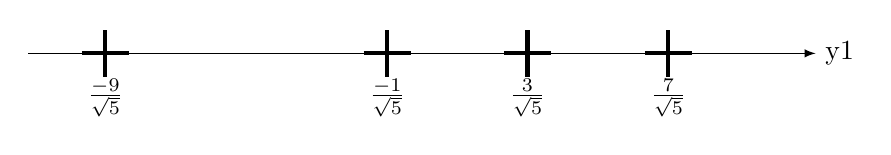
\begin{tikzpicture}
		\tikzstyle {point line} = [line width=0.15em]
										    
		\draw[-latex] (-5,0) -- (5,0) node[right]{y1};
								
		\draw[point line] (2.83, 0) -- (3.43, 0);	
		\draw[point line] (3.13, -0.3) -- (3.13, 0.3);
		\draw (3.13, -0.2) node [below] {$\frac{7}{\sqrt{5}}$};    	
						
		\draw[point line] (-0.74, 0) -- (-0.14, 0);	
		\draw[point line] (-0.44, -.3) -- (-0.44, .3);	
		\draw (-0.44, -0.2) node [below] {$\frac{-1}{\sqrt{5}}$};   
						
		\draw[point line] (1.04, 0) -- (1.64, 0);	
		\draw[point line] (1.34, -.3) -- (1.34, .3);	
		\draw (1.34, -0.2) node [below] {$\frac{3}{\sqrt{5}}$};   
						
		\draw[point line] (-4.32 , 0) -- (-3.72 , 0);	
		\draw[point line] (-4.02, -0.3) -- (-4.02,0.3 );	
		\draw (-4.02, -0.2) node [below] {$\frac{-9}{\sqrt{5}}$};   
							   		
	\end{tikzpicture}
\end{figure}

\section{Mathematics}

Assume a (MxN) matrix X as a set of N observations of M random variables such that each observation is a column in the matrix X. Furthermore, assume that each variable has zero mean meaning that each row of the matrix sums up to zero. Denote by $\sum_x$ the variance covariance matrix of the variables. Due to the zero mean condition, 

\begin{align*}
	\sum_x = XX^T 
\end{align*} 

Let $\phi_i, \phi_2, ..., \phi_m$ be the m orthonormal eigenvectors of $\sum_x$. Let P be defined as the matrix $[\phi_1^T, \phi_2^T, ..., \phi_m^T]^T$. Consider the following transformation, 

\begin{align*}
	Y = PX 
\end{align*}

It can be shown that the resulting variables are also zero-mean based. So, their variance covariance matrix can be written as,

\begin{align*}
	\sum_y & = YY^T       \\
	       & = (PX)(PX)^T \\
	       & = PXX^TP^T   \\
	       & = P\sum_xP^T \\           
\end{align*}

$\sum_x$ is symmetric and all symmetric matrices are diagonalized by a matrix of their orthonormal eigenvectors. Or more precisely,

\begin{align*}
	\sum_x = P^TDP 
\end{align*}

where D is a diagonal matrix. Upon substitution in the preceding equation,

\begin{align*}
	\sum_y = PP^TDPP^T 
\end{align*}

Since P is orthonormal, its transpose is its inverse and thus $PP^T = I$ which reduces $\sum_y$ to D.

\section{Kernel PCA}

Let X be $[x_1, x_2, ..., x_N]$ where each $x_i$ is an observation of M variables. Consider mapping each $x_i$ to $f(x_i)$ where $f$ is non-linear and may increase the dimensionality of each $x_i$. So,

\begin{align*}
    f(X) = [f(x_1), f(x_2), ..., f(x_N)]
\end{align*}

Now examine the variance covariance matrix of $f(X)$.

\begin{align*}
    \sum_f &= \frac{1}{N}f(X)f(X)^T \\
           &= \frac{1}{N}[f(x_1), f(x_2), ..., f(x_N)]\begin{pmatrix}
               f(x_1^T) \\
               f(x_2^T) \\
               ... \\
               f(x_N^T) 
           \end{pmatrix} \\
           &= \frac{1}{N} \sum_{i = 1}^{N} f(x_i)f(x_i^T) \\
\end{align*}

To find principal components, eigenvalues and eigenvectors of the variance covariance matrix must be found out. since there are N eigenvalue, eigenvector pairs, they will be subscripted by j.

\begin{align*}
    \lambda_j\phi_j &= \sum_f\phi_j\\
    \lambda_j\phi_j &= \frac{1}{N} \sum_{i = 1}^{N} f(x_i)f(x_i^T)\phi_j \\
\end{align*}

Since $f(x_i^T)\phi_j = \vec{f(x_i)}.\vec{\phi_j}$ is just a scalar, the equation can be simplified to,

\begin{align*}
    \phi_j &= \sum_{i = 1}^{N} \frac{\vec{f(x_i)}.\vec{\phi_j}}{N\lambda_j}f(x_i) \\
\end{align*}

Substituting $\frac{\vec{f(x_i)}.\vec{\phi_j}}{N\lambda_j}$ = $a_{ij}$, the equation becomes,

\begin{align*}
    \phi_j = \sum_{i = 1}^{N} a_{ij} f(x_i) 
\end{align*} 

This equation reveas that the principal components are linear combinations of the observations.

\begin{align*}
    \phi_j = a_{1j}f(x_1) + a_{2j}f(x_2) + ... + a_{Nj}f(x_N) \\ 
\end{align*}

Taking dot products by $f(x_1), f(x_2) ... f(x_N)$ successively,

\begin{align*}
       \vec{f(x_1)}.\vec{\phi_j} &= a_{1j}\vec{f(x_1)}.\vec{f(x_1)} + a_{2j}\vec{f(x_1)}.\vec{f(x_2)} + ... + a_{Nj}\vec{f(x_1)}.\vec{f(x_N)} \\
\vec{f(x_2)}.\vec{\phi_j} &= a_{1j}\vec{f(x_2)}.\vec{f(x_1)} + a_{2j}\vec{f(x_2)}.\vec{f(x_2)} + ... + a_{Nj}\vec{f(x_2)}.\vec{f(x_N)} \\ 
    ... &= ... \\
    \vec{f(x_N)}.\vec{\phi_j} &= a_{1j}\vec{f(x_N)}.\vec{f(x_1)} + a_{2j}\vec{f(x_N)}.\vec{f(x_2)} + ... + a_{Nj}\vec{f(x_N)}.\vec{f(x_N)}
\end{align*}

In matrix form, these equation look like,

\begin{align*}
    \begin{pmatrix}
        \vec{f(x_1)}.\vec{\phi_j} \\
        \vec{f(x_2)}.\vec{\phi_j} \\
        ... \\
        \vec{f(x_N)}.\vec{\phi_j} 
    \end{pmatrix} = \begin{pmatrix}
        \vec{f(x_1)}.\vec{f(x_1)} & \vec{f(x_1)}.\vec{f(x_2)} & ... &  \vec{f(x_1)}.\vec{f(x_N)} \\
        \vec{f(x_2)}.\vec{f(x_1)} & \vec{f(x_2)}.\vec{f(x_2)} & ... &  \vec{f(x_2)}.\vec{f(x_N)} \\
        ... \\
        \vec{f(x_N)}.\vec{f(x_1)} & \vec{f(x_N)}.\vec{f(x_2)} & ... &  \vec{f(x_N)}.\vec{f(x_N)} \\
    \end{pmatrix} \begin{pmatrix}
        a_{1j} \\
        a_{2j} \\
        ... \\
        a_{Nj} \\
    \end{pmatrix}
\end{align*}

The first matrix on the right is a NxN matrix. Denote it by the kernel matrix: K. For every term on the left hand side matrix use the fact that $\vec{f(x_i)}.\vec{\phi_j} = N\lambda_j a_{ij}$.

\begin{align*}
    N\lambda_j \begin{pmatrix}
        a_{1j} \\
        a_{2j} \\
        ... \\
        a_{Nj} \\
    \end{pmatrix} = K \begin{pmatrix}
        a_{1j} \\
        a_{2j} \\
        ... \\
        a_{Nj} \\
    \end{pmatrix}
\end{align*}

It is apparent that $N\lambda_j, [a_{1j}, a_{2j}, ..., a_{Nj}]^T \forall j \in [1, N]$are eigenvalue, eigenvector pairs for the matrix K. The PCA transform for $f(X)$ can be written as,

\begin{align*}
    Y &= \begin{pmatrix}
        \phi_1^T \\
        \phi_2^T \\
        ... \\
        \phi_N^T \\
    \end{pmatrix} f(X) \\
      &= \begin{pmatrix}
        \phi_1^T \\
        \phi_2^T \\
        ... \\
        \phi_N^T \\
    \end{pmatrix} [f(x_1), f(x_2), ..., f(x_N)] \\
      &= \begin{pmatrix}
          \vec{\phi_1}.\vec{f(x_1)} & \vec{\phi_1}.\vec{f(x_2)} & ... & \vec{\phi_1}.\vec{f(x_N)} \\
          \vec{\phi_2}.\vec{f(x_1)} & \vec{\phi_2}.\vec{f(x_2)} & ... & \vec{\phi_2}.\vec{f(x_N)} \\
          ... \\
          \vec{\phi_N}.\vec{f(x_1)} & \vec{\phi_N}.\vec{f(x_2)} & ... & \vec{\phi_N}.\vec{f(x_N)} \\
\end{pmatrix}       
\end{align*} 

Using the relation $\vec{f(x_i)}.\vec{\phi_j} = N\lambda_j a_{ij}$,

\begin{align*}
    Y &= \begin{pmatrix}
          N\lambda_1 a_{11} & N\lambda_1 a_{21} & ... & N\lambda_1 a_{N1} \\ 
          N\lambda_2 a_{12} & N\lambda_2 a_{22} & ... & N\lambda_2 a_{N2} \\ 
          ... \\
          N\lambda_N a_{1N} & N\lambda_N a_{2N} & ... & N\lambda_N a_{NN} \\ 
\end{pmatrix} \\
    &=  N\begin{pmatrix}
          \lambda_1 a_{11} & \lambda_1 a_{21} & ... & \lambda_1 a_{N1} \\ 
          \lambda_2 a_{12} & \lambda_2 a_{22} & ... & \lambda_2 a_{N2} \\ 
          ... \\
          \lambda_N a_{1N} & \lambda_N a_{2N} & ... & \lambda_N a_{NN} \\ 
\end{pmatrix}      
\end{align*} 

This is the kernel trick for PCA where it is not required to explicit map each point to higher dimensions whcich may be computationally expensive. PCA transformation in nonlinear higher dimensions can be calculated by performing the following steps in the order below. 

\begin{itemize}
    \item Choose a kernel $ k(x_i, x_j) = \vec{f(x_i)}.\vec{f(x_j)}$.
    \item Calculate kernel matrix K = $\begin{pmatrix}
        k(x_1, x_1) & k(x_1, x_2) & ... & k(x_1, x_N) \\
        k(x_2, x_1) & k(x_2, x_2) & ... & k(x_2, x_N) \\
        ... \\
        k(x_N, x_1) & k(x_N, x_2) & ... & k(x_N, x_N) \\
    \end{pmatrix}$.
    \item Find the eigenvalue, eigenvalue pairs of K.
    \item Use eigenvalue, eigenvector pairs to calcuate the kernel PCA transform as shown above.
    \item Do dimensinality reduction as appropriate.  
\end{itemize}

\section{Assumptions and Limitations}


\end{document}